\section{Scenario}\label{4_6_scenario}
To have a better understanding regarding the interplay of the several components a generic scenario workflow will be given from the point of view of the user:

The user raises the hands over her head to start the application. She is now instructed on how to interact with elements on  the screen, e.g. clicking and scrolling. After being confident with this, she selects her user profile to load the appropriate exercises and leads her to the stage selection. She selects the first stage since all others are currently locked. Now she is in the exercise menu. In here she clicks on the \textit{stage information} button, which gives her an introduction into the stage. After confirming that she has read the introduction the first exercise becomes unlocked and she selects it. After that she decides to train her left leg first in the side selection. An exercise introduction screen is following, which shows specific information about the execution. After reading the introduction she feels ready to counter the exercise. Therefore she goes into the starting position and starts the exercise by clicking the start button. The screen changes and all relevant elements are shown for the exercise execution. She performs every repetition of the exercise successfully. After finishing these the system leads her to the exercise summary screen, which shows her the performance of the just executed exercise. In here she can now decide to return to the main menu or go on and start the training for the other body side. This procedure is also visualized in Figure \ref{fig:scenarioWorkflow} below.
\begin{comment}
\todo{-maybe just user view scenario}
To have a better understanding regarding the interplay of the several components a generic scenario workflow will be given.
The user starts with an engagement gesture like raising her hand over the head to convey that the system initially recognises and responds to a user action. After that a tutorial about the interaction with the system will be given that covers clicking and scrolling techniques. Now she's confident with the system interaction and can select a profile in the user select to train. This loads the profile which leads to the stage selection menu. In here she can select a stage, whereas initially the first one is can be selected and the others have to be unlocked by successfully accomplishing all exercises in the preview stage. Selecting a stage leads to the exercise menu. In here she has to read initially the stage introduction to become a basic understanding about the exercises in here. After reading this, it unlocks the first exercise. Selecting an exercise leads to the side selection, where the user has to choose the side she wants to train for this exercise. This is followed by an introduction of the exercise, in which is explained how to perform it correctly. If the user is ready, she should stay in a starting position to be able to start the exercise execution. In here she find all relevant elements to perform the exercise, like indicators for the time, repetitions, confidence and a checklist, which helps her to correctly execute the exercise. After successfully executing the exercise, a summary is shown which summarizes the user performance. Then she can return to the main menu or directly approach the next exercise. A stage summary gives an overview about all exercises with average performance parameters.
\end{comment}

\begin{figure}[htb]
	\centering
	\begin{minipage}[t]{1\linewidth}
		\centering
		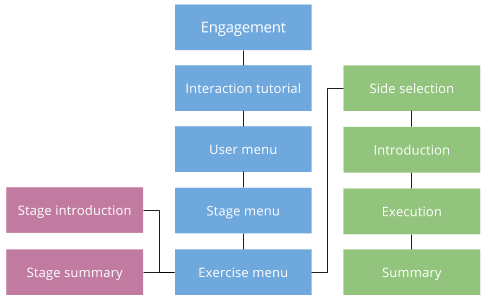
\includegraphics[width=1\linewidth]{Pictures/conceptScenarioFlow2}
		\caption{Scenario workflow}
		\label{fig:scenarioWorkflow}
	\end{minipage}
\end{figure}